\label{appendix}
Los siguientes experimentos fueron realizados para poder comprobar 
que la distribución de datos tanto del \textit{dataset} de 
entrenamiento como el de \textit{testing} eran diferentes, 
generando un \textit{overfitting} accidental en la experimentación 
general. 

\section{Experimentación A (training/ validation/ testing)}

Una vez de terminado la creación de los \textit{bounding boxes} de parte 
del experto, se procedió a realizar la comprobación del modelo en base a 
los datos de \textit{testing}. Los estadísticos resultantes del \textit{testing} 
fueron los mostrados en la tabla \ref{table:Anexo2}.
\begin{table}[h!]
\centering
\begin{tabular}{|l|l|l|l|l|}
\hline
\multicolumn{1}{|c|}{\textit{Loss}} & \textit{\begin{tabular}[c]{@{}c@{}}Balanced\\Accuracy\end{tabular}}  & \multicolumn{1}{c|}{\textit{F1-weighted}} & \multicolumn{1}{c|}{\textit{Precision}} & \multicolumn{1}{c|}{\textit{Recall}} \\ \hline
2.7014          & 46.50\%                          & 41.46\%                  & 50.28\%                         & 49.54\%                      \\ \hline
\end{tabular}
\caption{Estadísticos obtenidos del experimento \#A}
\label{table:Anexo2}
\end{table}

Los estadísticos obtenidos empeoraron en comparación con los datos de 
entrenamiento. Para confirmar las sospechas de un posible 
\textit{overfitting}, se revisaron las gráficas de pérdida a través de 
las épocas, que se pueden ver en la imagen \ref{fig:losses3}.

\begin{figure}[h!]
\footnotesize
\centering
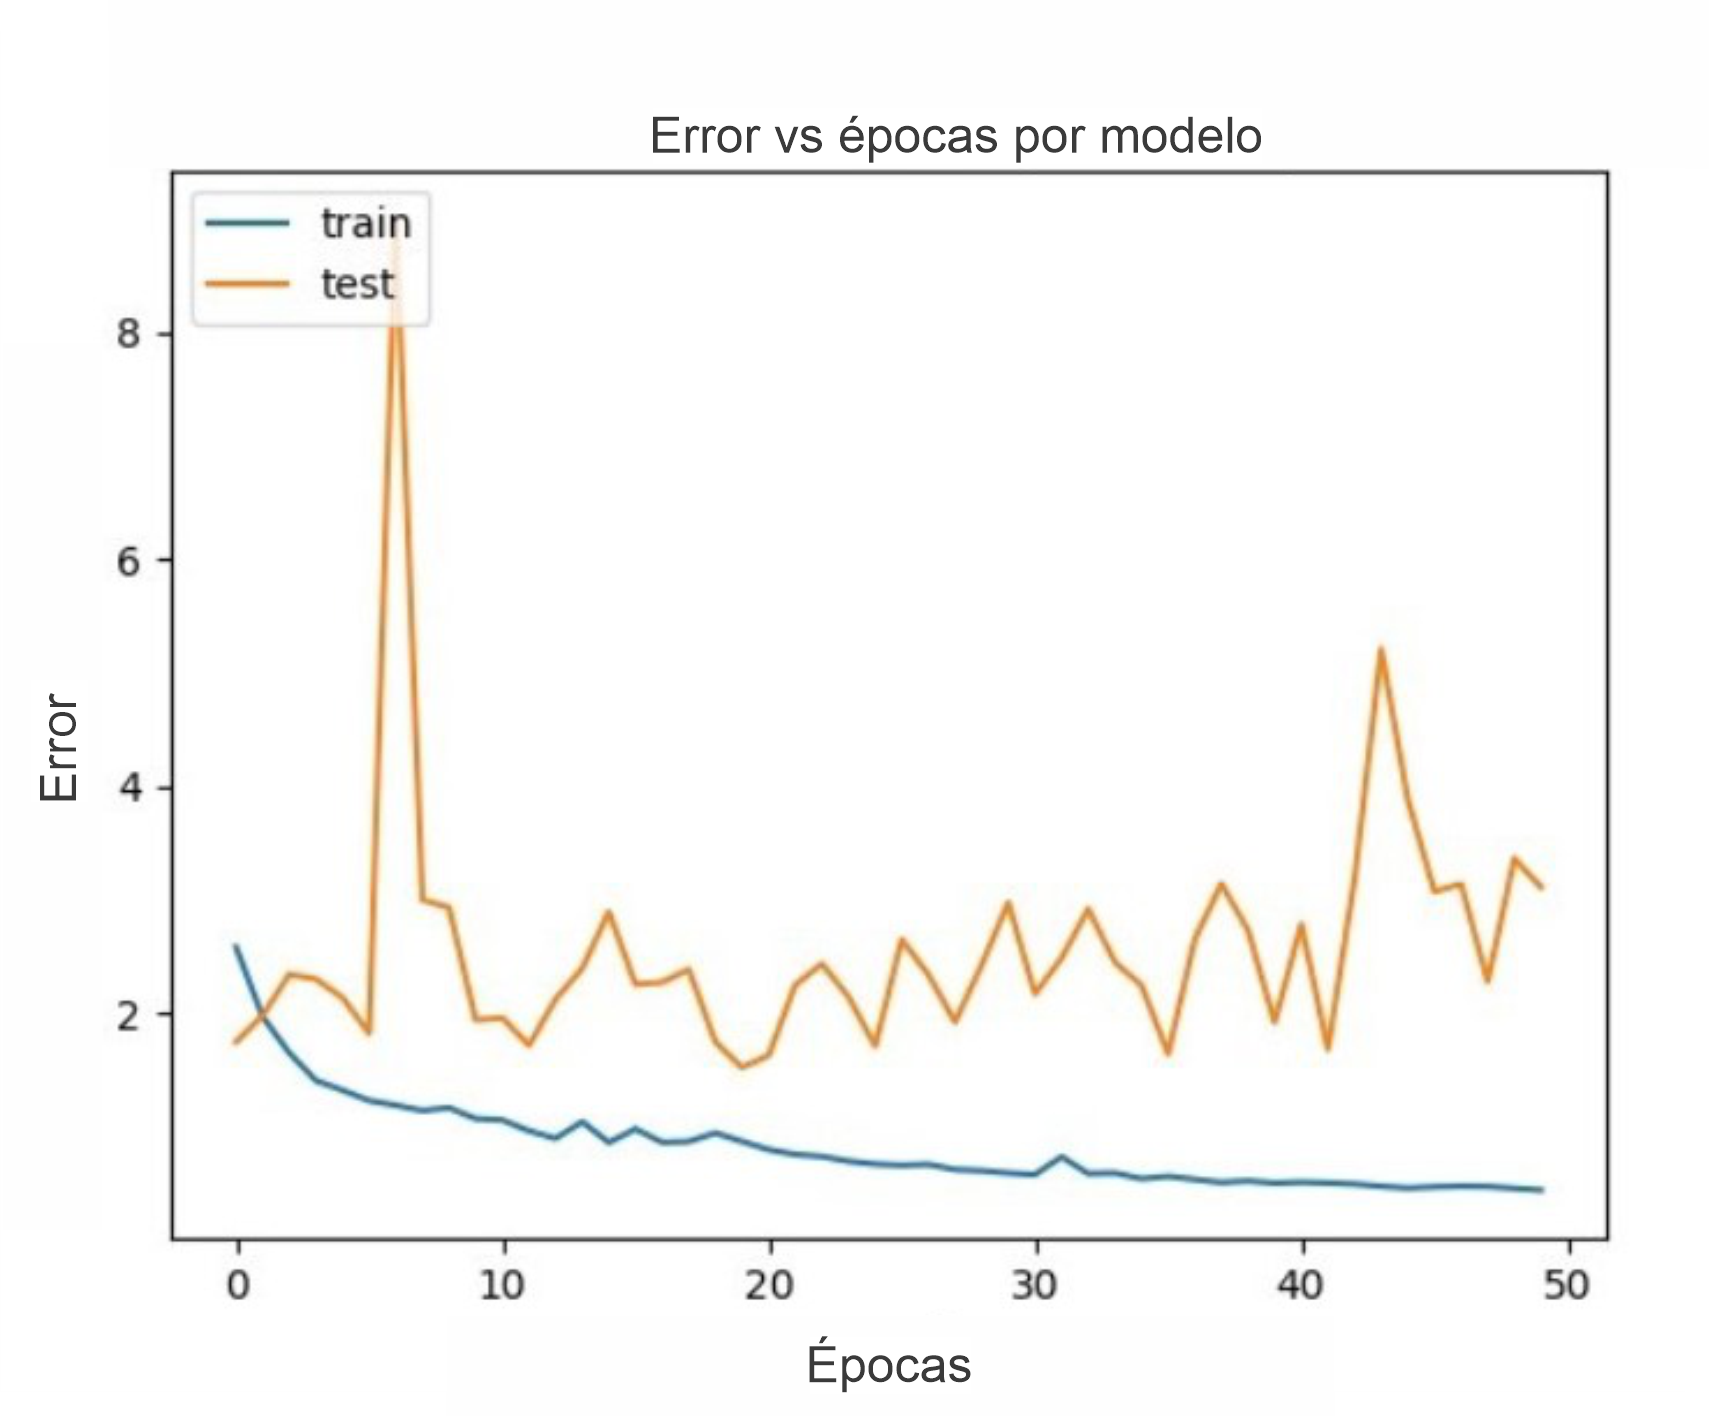
\includegraphics[width=1\textwidth]{images/loss3.png}
\caption{Gráfica comparativa de la perdida de entrenamiento y \textit{testing}}
\label{fig:losses3}
\end{figure}

Una vez más, la gráfica muestra un posible caso de \textit{overfitting} de los 
datos y, aún peor, la gráfica de error indica un aumento en lugar de una disminución 
a lo largo de las épocas. Para evaluar de manera más detallada los resultados, 
se revisó la matriz de confusión generada, la cual se muestra en la tabla 
\ref{table:Matrix1}.
\newpage
\begin{table}[h!]
\footnotesize
\begin{tabular}{|c|c|c|c|c|c|c|c|}
\hline
                                                                  & \begin{tabular}[c]{@{}c@{}}Albacore\\ Tuna\end{tabular} & \begin{tabular}[c]{@{}c@{}}Bigeye\\ Tuna\end{tabular} & \begin{tabular}[c]{@{}c@{}}Dolphin\\Fish\end{tabular} & \begin{tabular}[c]{@{}c@{}}Moonfish\\ (LAG)\end{tabular} & Shark   & \begin{tabular}[c]{@{}c@{}}Yellowfin\\ Tuna\end{tabular} & Other   \\ \hline
\textit{\begin{tabular}[c]{@{}c@{}}Albacore\\ Tuna\end{tabular}}  & 94.26\%                                                 & 00.78\%                                               & 00.00\%     & 00.00\%                                                  & 00.78\% & 01.57\%                                                  & 02.61\% \\ \hline
\textit{\begin{tabular}[c]{@{}c@{}}Bigeye\\ Tuna\end{tabular}}    & 88.23\%                                                 & 03.07\%                                               & 00.00\%     & 00.00\%                                                  & 00.51\% & 00.77\%                                                  & 07.42\% \\ \hline
\begin{tabular}[c]{@{}c@{}}Dolphin\\Fish\end{tabular}                                              & 35.00\%                                                 & 00.00\%                                               & 50.00\%     & 00.00\%                                                  & 00.00\% & 05.00\%                                                  & 10.00\% \\ \hline
\textit{\begin{tabular}[c]{@{}c@{}}Moonfish\\ (LAG)\end{tabular}} & 25.42\%                                                 & 00.00\%                                               & 03.39\%     & 57.63\%                                                  & 06.78\% & 00.00\%                                                  & 06.78\% \\ \hline
\textit{Shark}                                                    & 50.38\%                                                 & 00.76\%                                               & 00.00\%     & 00.00\%                                                  & 38.93\% & 04.58\%                                                  & 05.34\% \\ \hline
\textit{\begin{tabular}[c]{@{}c@{}}Yellowfin\\ Tuna\end{tabular}} & 33.33\%                                                 & 09.52\%                                               & 00.00\%     & 00.00\%                                                  & 00.00\% & 38.09\%                                                  & 19.05\% \\ \hline
\textit{Other}                                                    & 23.78\%                                                 & 01.22\%                                               & 01.22\%     & 00.00\%                                                  & 00.00\% & 00.00\%                                                  & 73.78\% \\ \hline
\end{tabular}
\caption{Matriz de confusión generada por las imágenes de \textit{testing} en porcentajes}
\label{table:Matrix1}
\end{table}


En la tabla se puede observar que la red tiende a predecir que los ejemplares 
pertenecen a la primera especie, lo que sugiere que está sobre aprendiendo de esta 
clase, posiblemente debido a la mayor cantidad de datos disponibles. A pesar de que 
esta hipótesis podría parecer plausible, no es la correcta, como se verá en los siguientes experimentos.

\section{Experimentación B (training/ validation/ testing con \textit{unfreeze})}

Para intentar reducir el posible \textit{overfitting}, se decidió quitar el 
\textit{freeze} de los dos últimos bloques de capas convolucionales del modelo pre-entrenado, 
permitiendo así que el modelo aprenda más patrones dentro de las imágenes. Después de esta 
modificación, se obtuvieron los resultados que se muestran en la tabla \ref{table:Results3}.

\begin{table}[h!]
\centering
\begin{tabular}{|l|l|l|l|l|l|}
\hline
                                                                            & \multicolumn{1}{c|}{\textit{Loss}} & \textit{\begin{tabular}[c]{@{}c@{}}Balanced\\Accuracy\end{tabular}} & \multicolumn{1}{c|}{\textit{F1-weighted}} & \multicolumn{1}{c|}{\textit{Precision}} &  \multicolumn{1}{c|}{\textit{Recall}} \\ \hline
\textit{\begin{tabular}[c]{@{}l@{}}Bloque 7 \\ unfreezed\end{tabular}}      & 4.1616                              & 51.71\%                                 & 42.23\%                           & 51.17\%                                  & 50.92\%                               \\ \hline
\textit{\begin{tabular}[c]{@{}l@{}}Bloques 6 y 7 \\ unfreezed\end{tabular}} & 3.1206                              & 19.56\%                                 & 28.97\%                           & 40.58\%                                  & 33.90\%                               \\ \hline
\end{tabular}
\caption{Estadísticos obtenidos del experimento \#3}
\label{table:Results3}
\end{table}

De la misma manera, las gráficas de error y \textit{accuracy}, junto con las matrices de 
confusión resultaron similares al anterior experimento, por lo que surgió la duda acerca 
de si tal vez existía una incongruencia con la base de datos.
